\section{Постановка задачи}

\begin{frame}
    \frametitle{Схема плоской трещины гидроразрыва пласта (ГРП)}
    \centering
    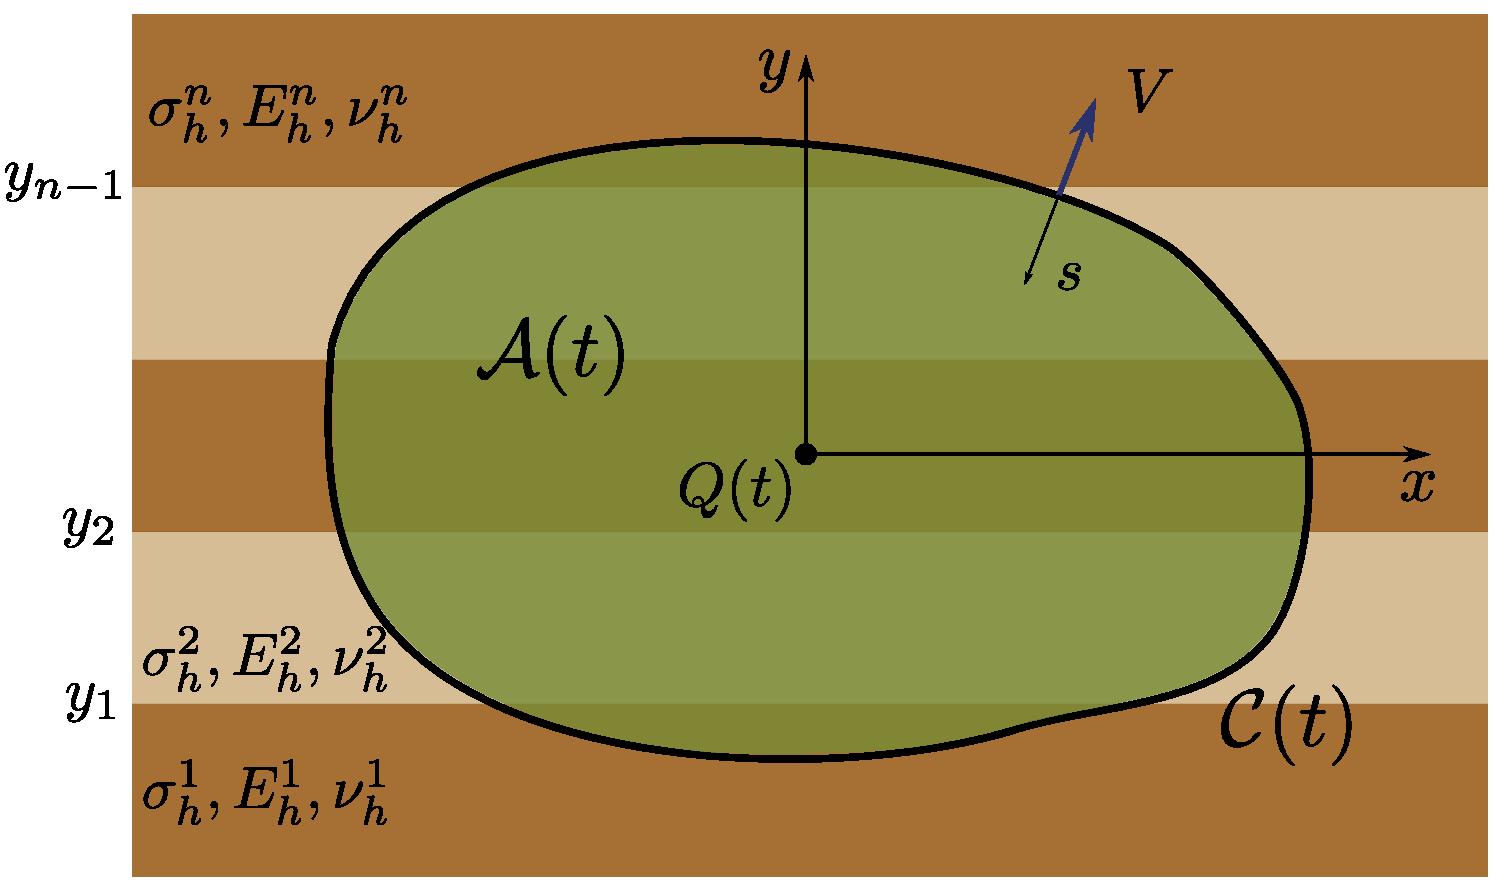
\includegraphics[width=0.8\textwidth]{fracture_scheme.pdf}
\end{frame}

\subsection{Определяющие уравнения}
\begin{frame}
    \frametitle{Модель плоской трещины ГРП}
    Уравнение Рейнольдса (закон сохранения массы)
    \begin{equation}
        \label{eq:reynolds_equation}
        \pd{w}{t} - \text{div} \left(\frac{w^3}{12\mu} \bigtriangledown \!p \right) + \frac{2C_L}{\sqrt{t-t_0(x,\, y)}}  = Q(t) \delta(x,\,y),
    \end{equation}

    Уравнение упругости
    \begin{equation}
        \label{eq:elasticity_equation}
        p(x,y,t) = \sigma_h(y) + \int\limits_{\mathcal{A}(t)} G(x,y;x',y')w(x',y',t) \dif x' \dif y',
    \end{equation}

    Граничные условия на движущемся фронте
    \begin{minipage}{0.49\textwidth}
        \begin{equation*}
            \lim_{s \to 0} \frac{w(s)}{s^{1/2}}=\frac{K'}{E'},
        \end{equation*}
    \end{minipage}
    \hfill
    \begin{minipage}{0.5\textwidth}
        \begin{equation}
            \lim_{s \to 0} \frac{w^3}{12\mu} \pd{p}{s}=0.
        \end{equation}
    \end{minipage}
\end{frame}

\begin{frame}
    \frametitle{Постановка задачи}
    В институте гидродинамики им. М. А. Лаврентьева СО РАН ранее был реализован симулятор ГРП Planar3D ILSA в предположении
    \begin{equation}
        \label{eq: heterogeneous_elasticity_equation}
        p(x,y,t) = \sigma_h(y) - \frac{E'}{8\pi}\int\limits_{\mathcal{A}(t)} \frac{w(x',y',t)}{[(x\!-\!x')^2+(y\!-\!y')^2]^{3/2}} \dif x' \dif y'.
    \end{equation}

    Целью данной работы является 
    \begin{itemize}
        \item реализация метода построения численной матрицы жесткости для слоистой среды с неоднородностью по модулям упругости и внедрение его в модель Planar3D ILSA,
        \item анализ влияния неоднородности модулей упругости на геометрию трещины ГРП,
        \item сравнение влияния неоднородности сжимающих напряжений и модулей упругости слоев на геометрию финальной трещины ГРП,
        \item анализ влияния тонких жестких пропластков на рост и раскрытие трещины ГРП.
    \end{itemize}
\end{frame}

\section{Численное построение матрицы упругости}
\begin{frame}
    \frametitle{Численное построение матрицы жесткости}
    Метод численного построения был предложен Энтони Пирсом \footfullcite{Peirce2001TheSF}.
    Для каждого слоя записываем уравнение равновесия для упругой изотропной среды
    \begin{equation}
        \label{eq:equilibrium}
        \sigma_{ij,j} + f_i = 0,
    \end{equation}
    закон Гука
    \begin{equation}		
        \sigma_{ij} = \lambda e_{kk}\delta_{ij} + 2G e_{ij}.
        \label{eq:hooke_law}
    \end{equation}
    На границе раздела слоев выполняется условие непрерывности компонент вектора смещений и нормальной нагрузки. Тогда ядро в интегральном соотношении~\eqref{eq:elasticity_equation}
    \begin{equation}
        \begin{split}
            G(x,y,x',y') & = \sigma_{zz}(x,y), \\
            \left[u_{z} \right]_{(x',y')} & = \left.u_{z-0} - u_{z+0}\right|_{(x',y')} = 1.
        \end{split}
    \end{equation}
\end{frame}

\begin{frame}
    \frametitle{Введение псевдо-границы}
    \begin{minipage}[t]{0.47\linewidth}
        \footnotesize{Условие точечного разрыва смещений}
        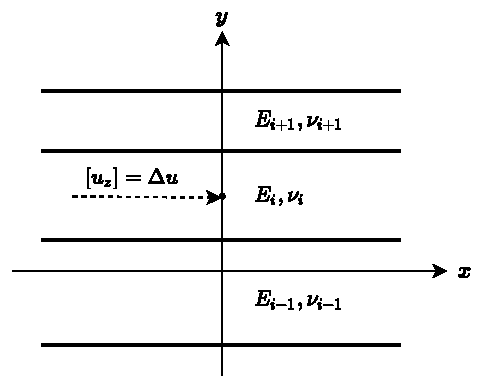
\includegraphics[width=\linewidth]{DD_point.pdf}
    \end{minipage}
    \hfill
    \begin{minipage}[t]{0.47\linewidth}
        \footnotesize{Введение дополнительной границы}
        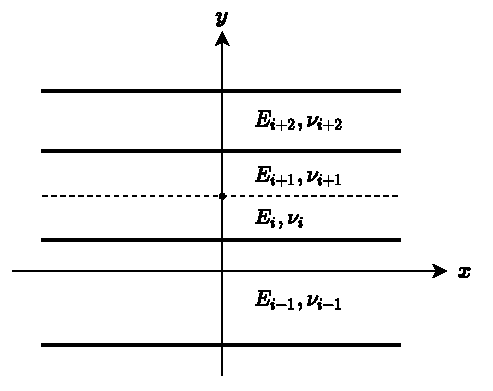
\includegraphics[width=\linewidth]{DD_point2.pdf}
    \end{minipage}
    Тогда $u_{z-0} - u_{z+0} = \Delta u$ может быть представлена в виде скачка смещений и напряжений на псевдо-границе $\left[ T \right] = T(y-0) - T(y+0)$, где $T = \left[\sigma_{yy} , \quad \sigma_{xy} , \quad \sigma_{yz} , \quad u_{y} , \quad u_{x} , \quad u_{z}\right]^T$.
\end{frame}

\begin{frame}
    \frametitle{Постановка в Фурье-образе}
    Записываем определяющие уравнения в виде
    \begin{equation}
        \label{eq:separate}
        \partial_{y} T = \mathbb{A}T,
    \end{equation}

    и применяя двумерное преобразование Фурье по координатам $x$ и $z$, получим
    \begin{equation}
        \label{eq:FT_system}
        \partial_y \hat{T} = \hat{\mathbb{A}} \hat{T}.
    \end{equation}
    Система \eqref{eq:FT_system} является ОДУ и решение зависит от 6 спектральных коэффициентов $A(m,n)$ (константы интегрирования)
    \begin{equation}
        \label{eq:fourier_solution}
        \hat{T} = \mathbb{Z}A.
    \end{equation}
    Связь между спектральными коэффициентами и значениями смещений и напряжений на границе слоя
    \begin{equation}
        A(m,n) = \mathbb{Z}^{-1}\hat{T}(y=y_i).
    \end{equation}
\end{frame}

\begin{frame}
    \frametitle{Связанная система уравнений для граничных значений}
    Из этих соотношений можно составить уравнения для определения компонент вектора смещения и напряжений на границе раздела слоев
    \begin{equation}
        \label{eq:coupled-system}
        \textbf{A}^i \hat{T}_{y=y_{i-1}} +
        \textbf{C}^i \hat{T}_{y=y_{i}} + 
        \textbf{B}^i \hat{T}_{y=y_{i+1}}
        = \textbf{D}^i,
    \end{equation}
    Ядро $G(x,y;x',y')$ интегрального соотношения~\eqref{eq:elasticity_equation} для слоистой среды
    \begin{equation}
        G(x,y;x',y') = G_\text{hom}(x,y;x',y') + G'(x,y;x',y'),
    \end{equation} 
    где
    \begin{equation}
        \begin{split}
            G_\text{hom}(x,y;x',y') & = - \frac{E'(y)}{8\pi [(x\!-\!x')^2+(y\!-\!y')^2]^{3/2}},\\
            G'(x,y;x',y') & = \Delta \sigma_{zz}(x,y),\\
            \left[u_{z} \right]_{(x',y')} & = \left.u_{z-0} - u_{z+0}\right|_{(x',y')} = 1.
        \end{split}
    \end{equation}
    где $\sigma_{zz}(x,y)$ находится из $\hat{\sigma}_{zz}(m,n)$ путем применения обратного дискретного преобразования Фурье.
\end{frame}

\begin{frame}
    \centering
    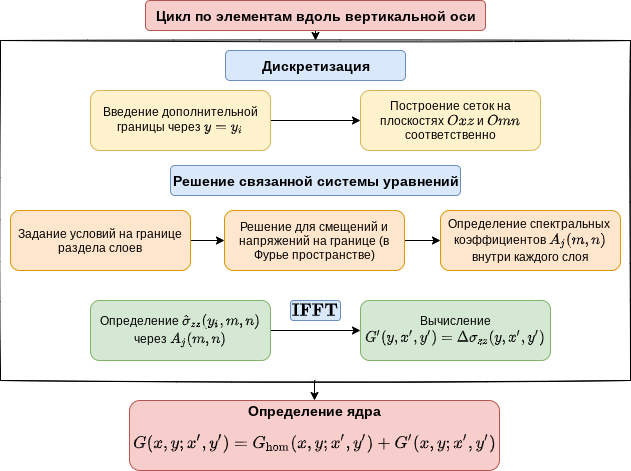
\includegraphics[width=0.9\textwidth]{scheme-layered.png}
\end{frame}


\section{Верификация и численные расчеты}

\begin{frame}[t]
    \frametitle{Верификация}
    \begin{columns}
        \begin{column}{0.4\textwidth}
            Численная сходимость метода
            \begin{enumerate}
                \item $E_{max} = \frac{||\mathbf{w}_h - \mathbf{w}||_{L_\infty}}{||\mathbf{w}||_{L_\infty}}$
                \item $E_2 = \frac{||\mathbf{w}_h - \mathbf{w}||_{L_2}}{||\mathbf{w}||_{L_2}}$
            \end{enumerate}
        \end{column}
        \begin{column}{0.55\textwidth}
            \centering
            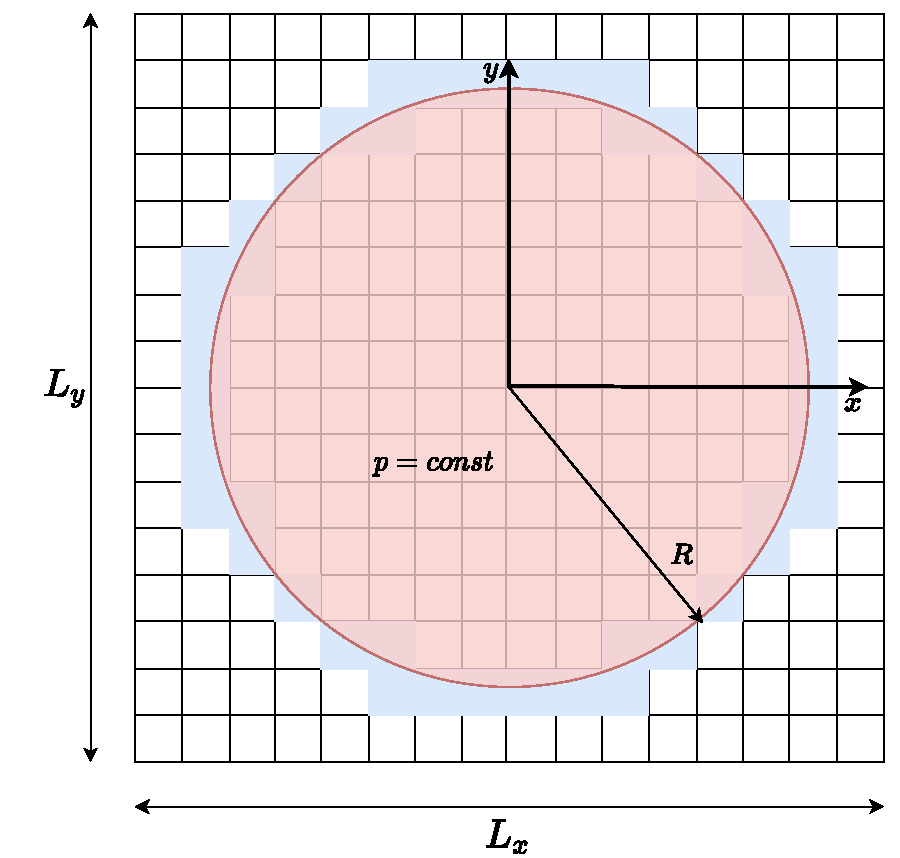
\includegraphics[width=\textwidth]{radial_fracture.pdf}
        \end{column}
    \end{columns}
\end{frame}

\begin{frame}
    \centering
    \begin{figure}
        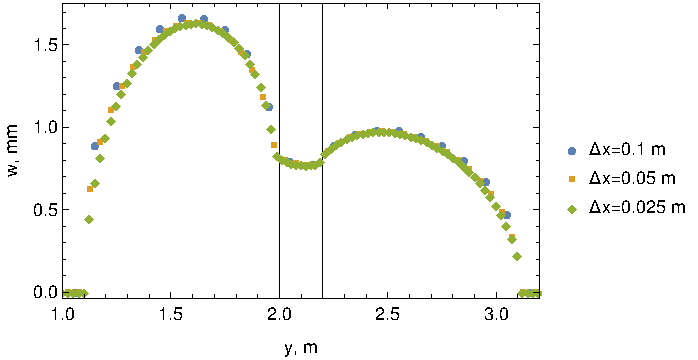
\includegraphics[width=0.7\textwidth]{static_accuracy.pdf}
        \caption{\footnotesize{Трехслойная среда, модуль Юнга и коэффициент Пуассона в слоях равны 1, 10, 2 GPa и 0.1, 0.4, 0.2 соответственно.}}
    \end{figure}

    \begin{tabular}{|c|c|c|}
        \hline
        $\Delta x, \text{м}$ & $E_{max}$ & $E_2$ \\
        \hline
        0.1                     & 0.129     & 0.059 \\
        \hline
        0.05                    & 0.096     & 0.028 \\
        \hline
        0.025 & --- & --- \\
        \hline
    \end{tabular}
\end{frame}

\begin{frame}
    \frametitle{Радиальная трещина, $E_\text{b} = E_\text{m} = E_\text{t} = 10$~GPa, $\nu_\text{b} = \nu_\text{m} = \nu_\text{t} = 0.22$}
    \begin{minipage}[t]{0.4\linewidth}
        \includegraphics[width=\linewidth]{Homogeneous/Figures/1/width_29.pdf}
    \end{minipage}
    \hfill
    \begin{minipage}[t]{0.57\linewidth}
        \includegraphics[width=\linewidth]{Homogeneous/Figures/1/w_y_29.pdf}
    \end{minipage}
\end{frame}

\begin{frame}
    \frametitle{Пласт с жестким нижним слоем, $E_\text{b} = 50$~GPa, $E_\text{m} = E_\text{t} = 10$~GPa, $\nu_\text{b} = \nu_\text{m} = \nu_\text{t} = 0.22$}
    \begin{minipage}[t]{0.4\linewidth}
        \includegraphics[width=\linewidth]{Heterogeneous/Figures/1/width_29.pdf}
    \end{minipage}
    \hfill
    \begin{minipage}[t]{0.57\linewidth}
        \includegraphics[width=\linewidth]{Heterogeneous/Figures/1/w_y_29.pdf}
    \end{minipage}
\end{frame}

\begin{frame}
    \frametitle{Пласт с сильной неоднородностью, $E_\text{b} = 100$~GPa, $E_\text{m} = E_\text{t} = 10$~GPa, $\nu_\text{b} = \nu_\text{m} = \nu_\text{t} = 0.22$}
    \begin{minipage}[t]{0.4\linewidth}
        \includegraphics[width=\linewidth]{Heterogeneous/Figures/2/width_29.pdf}
    \end{minipage}
    \hfill
    \begin{minipage}[t]{0.57\linewidth}
        \includegraphics[width=\linewidth]{Heterogeneous/Figures/2/w_y_29.pdf}
    \end{minipage}
\end{frame}

\begin{frame}
    \frametitle{Пласт с сильной неоднородностью, $E_\text{m} = 10$~GPa, $E_\text{b} = E_\text{t} = 100$~GPa, $\nu_\text{b} = \nu_\text{m} = \nu_\text{t} = 0.22$}
    \begin{minipage}[t]{0.4\linewidth}
        \includegraphics[width=\linewidth]{Heterogeneous/Figures/3_3/width_29.pdf}
    \end{minipage}
    \hfill
    \begin{minipage}[t]{0.57\linewidth}
        \includegraphics[width=\linewidth]{Heterogeneous/Figures/3_3/w_y_29.pdf}
    \end{minipage}
\end{frame}

\begin{frame}
    \frametitle{$E_\text{b} = 20$~GPa, $E_\text{m} = E_\text{t} = 10$~GPa, $\nu_\text{b} = \nu_\text{m} = \nu_\text{t} = 0.22$, $\sigma_{h,\text{b}} = 30$~MPa, $\sigma_{h,\text{m}} = \sigma_{h,\text{t}} = 30.5$~MPa}
    \begin{minipage}[t]{0.4\linewidth}
        \includegraphics[width=\linewidth]{Heterogeneous/Figures/3/width_29.pdf}
    \end{minipage}
    \hfill
    \begin{minipage}[t]{0.57\linewidth}
        \includegraphics[width=\linewidth]{Heterogeneous/Figures/3/w_y_29.pdf}
    \end{minipage}
\end{frame}

\begin{frame}
    \frametitle{$E_\text{b} = 40$~GPa, $E_\text{m} = E_\text{t} = 10$~GPa, $\nu_\text{b} = \nu_\text{m} = \nu_\text{t} = 0.22$, $\sigma_{h,\text{b}} = 30$~MPa, $\sigma_{h,\text{m}} = \sigma_{h,\text{t}} = 30.5$~MPa}
    \begin{minipage}[t]{0.4\linewidth}
        \includegraphics[width=\linewidth]{Heterogeneous/Figures/3_2/width_29.pdf}
    \end{minipage}
    \hfill
    \begin{minipage}[t]{0.57\linewidth}
        \includegraphics[width=\linewidth]{Heterogeneous/Figures/3_2/w_y_29.pdf}
    \end{minipage}
\end{frame}

\begin{frame}
    \frametitle{Пласт с включением тонкого слоя, $d=10$~м. , $k=\frac{E_d}{E}=5$}
    \begin{minipage}[t]{0.4\linewidth}
        \includegraphics[width=\linewidth]{Heterogeneous/Figures/4/width_29.pdf}
    \end{minipage}
    \hfill
    \begin{minipage}[t]{0.57\linewidth}
        \includegraphics[width=\linewidth]{Heterogeneous/Figures/4/w_y_29.pdf}
    \end{minipage}
\end{frame}

\begin{frame}
    \frametitle{Пласт с включением двух тонких пропластков, $d=10$~м. , $k=\frac{E_d}{E}=5$}
    \begin{minipage}[t]{0.4\linewidth}
        \includegraphics[width=\linewidth]{Heterogeneous/Figures/5/width_29.pdf}
    \end{minipage}
    \hfill
    \begin{minipage}[t]{0.57\linewidth}
        \includegraphics[width=\linewidth]{Heterogeneous/Figures/5/w_y_29.pdf}
    \end{minipage}
\end{frame}